% questions.tex —— 2005 年·普通高等学校招生考试·辽宁卷 · 题目内容片段（无答案）
% 由 tools/generate_projects.py 依来源总账自 2005/2005_数学真题_辽宁_试题.md 生成，勿手改（改源 MD 后重跑）

\gkpart{一、选择题（本大题共 12 小题，每小题 5 分，共 60 分。在每小题给出的四个选项中，只有一项是符合题目要求的）}

\begin{question}
\gkti{1}复数 $z = \dfrac{-1+\mathrm{i}}{1+\mathrm{i}} - 1$ 在复平面内，$z$ 所对应的点在\mbox{（　　）}

\begin{gkopts}(4)
\task A．第一象限
\task B．第二象限
\task C．第三象限
\task D．第四象限
\end{gkopts}

\end{question}
\begin{question}
\gkti{2}极限 $\lim\limits_{x \to x_0} f(x)$ 存在是函数 $f(x)$ 在点 $x = x_0$ 处连续的\mbox{（　　）}

\begin{gkopts}(2)
\task A．充分而不必要的条件
\task B．必要而不充分的条件
\task C．充要条件
\task D．既不充分也不必要的条件
\end{gkopts}

\end{question}
\begin{question}
\gkti{3}设袋中有 80 个红球，20 个白球，若从袋中任取 10 个球，则其中恰有 6 个红球的概率为\mbox{（　　）}

\begin{gkopts}(1)
\task A．$\dfrac{\mathrm{C}_{80}^{4} \cdot \mathrm{C}_{10}^{6}}{\mathrm{C}_{100}^{10}}$
\task B．$\dfrac{\mathrm{C}_{80}^{6} \cdot \mathrm{C}_{10}^{4}}{\mathrm{C}_{100}^{10}}$
\task C．$\dfrac{\mathrm{C}_{80}^{4} \cdot \mathrm{C}_{20}^{6}}{\mathrm{C}_{100}^{10}}$
\task D．$\dfrac{\mathrm{C}_{80}^{6} \cdot \mathrm{C}_{20}^{4}}{\mathrm{C}_{100}^{10}}$
\end{gkopts}

\end{question}
\begin{question}
\gkti{4}已知 $m$、$n$ 是两条不重合的直线，$\alpha$、$\beta$、$\gamma$ 是三个两两不重合的平面，给出下列四个命题：
① 若 $m \perp \alpha$，$m \perp \beta$，则 $\alpha \parallel \beta$；
② 若 $\alpha \perp \gamma$，$\beta \perp \alpha$，则 $\alpha \parallel \beta$；
③ 若 $m \subset \alpha$，$n \subset \beta$，$m \parallel n$，则 $\alpha \parallel \beta$；
④ 若 $m$、$n$ 是异面直线，$m \subset \alpha$，$m \parallel \beta$，$n \subset \beta$，$n \parallel \alpha$，则 $\alpha \parallel \beta$．
其中真命题是\mbox{（　　）}

\begin{gkopts}(4)
\task A．①和②
\task B．①和③
\task C．③和④
\task D．①和④
\end{gkopts}

\end{question}
\begin{question}
\gkti{5}函数 $y = \ln\left(x + \sqrt{x^2+1}\right)$ 的反函数是\mbox{（　　）}

\begin{gkopts}(1)
\task A．$y = \dfrac{\mathrm{e}^x + \mathrm{e}^{-x}}{2}$
\task B．$y = -\dfrac{\mathrm{e}^x + \mathrm{e}^{-x}}{2}$
\task C．$y = \dfrac{\mathrm{e}^x - \mathrm{e}^{-x}}{2}$
\task D．$y = -\dfrac{\mathrm{e}^x - \mathrm{e}^{-x}}{2}$
\end{gkopts}

\end{question}
\begin{question}
\gkti{6}若 $\log_{2a}\dfrac{1+a^2}{1+a} < 0$，则 $a$ 的取值范围是\mbox{（　　）}

\begin{gkopts}(2)
\task A．$\left(\dfrac{1}{2}, +\infty\right)$
\task B．$(1, +\infty)$
\task C．$\left(\dfrac{1}{2}, 1\right)$
\task D．$\left(0, \dfrac{1}{2}\right)$
\end{gkopts}

\end{question}
\begin{question}
\gkti{7}在 $\mathbf{R}$ 上定义运算 $\otimes$：$x \otimes y = x(1-y)$．若不等式 $(x-a) \otimes (x+a) < 1$ 对任意实数 $x$ 成立，则\mbox{（　　）}

\begin{gkopts}(2)
\task A．$-1 < a < 1$
\task B．$0 < a < 2$
\task C．$-\dfrac{1}{2} < a < \dfrac{3}{2}$
\task D．$-\dfrac{3}{2} < a < \dfrac{1}{2}$
\end{gkopts}

\end{question}
\begin{question}
\gkti{8}若钝角三角形三内角的度数成等差数列，且最大边长与最小边长的比值为 $m$，则 $m$ 的范围是\mbox{（　　）}

\begin{gkopts}(4)
\task A．$(1, 2)$
\task B．$(2, +\infty)$
\task C．$[3, +\infty)$
\task D．$(3, +\infty)$
\end{gkopts}

\end{question}
\begin{question}
\gkti{9}若直线 $2x - y + c = 0$ 按向量 $\vec{a} = (1, -1)$ 平移后与圆 $x^2 + y^2 = 5$ 相切，则 $c$ 的值为\mbox{（　　）}

\begin{gkopts}(2)
\task A．$8$ 或 $-2$
\task B．$6$ 或 $-4$
\task C．$4$ 或 $-6$
\task D．$2$ 或 $-8$
\end{gkopts}

\end{question}
\begin{question}
\gkti{10}已知 $y = f(x)$ 是定义在 $\mathbf{R}$ 上的单调函数，实数 $x_1 \neq x_2$，$\lambda \neq -1$，$\alpha = \dfrac{x_1 + \lambda x_2}{1+\lambda}$，$\beta = \dfrac{x_2 + \lambda x_1}{1+\lambda}$．若 $|f(x_1) - f(x_2)| < |f(\alpha) - f(\beta)|$，则\mbox{（　　）}

\begin{gkopts}(2)
\task A．$\lambda < 0$
\task B．$\lambda = 0$
\task C．$0 < \lambda < 1$
\task D．$\lambda \geqslant 1$
\end{gkopts}

\end{question}
\begin{question}
\gkti{11}已知双曲线的中心在原点，离心率为 $\sqrt{3}$．若它的一条准线与抛物线 $y^2 = 4x$ 的准线重合，则该双曲线与抛物线 $y^2 = 4x$ 的交点到原点的距离是\mbox{（　　）}

\begin{gkopts}(2)
\task A．$2\sqrt{3} + \sqrt{6}$
\task B．$\sqrt{21}$
\task C．$\sqrt{18 + 12\sqrt{2}}$
\task D．$21$
\end{gkopts}

\Needspace{0.4\textheight}
\end{question}
\begin{question}
\gkti{12}一给定函数 $y = f(x)$ 的图象在下列图中，并且对任意 $a_1 \in (0, 1)$，由关系式 $a_{n+1} = f(a_n)$ 得到的数列 $\{a_n\}$ 满足 $a_{n+1} > a_n$（$n \in \mathbf{N}^*$），则该函数的图象是\mbox{（　　）}
\nopagebreak[4]
\begin{center}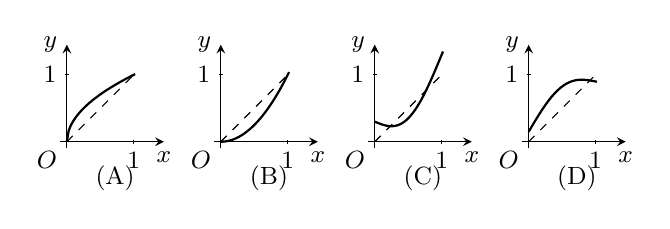
\begin{tikzpicture}[>=stealth, scale=0.85]
  % 四个候选图象：(A) 恒在 y=x 上方、(B) 恒在下方、(C) 先上后下、(D) 先下后上
  \foreach \dx/\name in {0/(A), 2.3/(B), 4.6/(C), 6.9/(D)}{
    \begin{scope}[shift={(\dx,0)}]
      \draw[->] (-0.1,0) -- (1.45,0) node[below] {\small $x$};
      \draw[->] (0,-0.1) -- (0,1.45) node[left] {\small $y$};
      \node[below left] at (0,0) {\small $O$};
      \draw[dashed] (0,0) -- (1.05,1.05);
      \draw (-0.03,1) -- (0.03,1) node[left=1pt] {\small $1$};
      \draw (1,-0.03) -- (1,0.03) node[below=1pt] {\small $1$};
      \node[below] at (0.72,-0.22) {\small \name};
    \end{scope}
  }
  % (A) y = sqrt(x)
  \begin{scope}[shift={(0,0)}]
    \draw[thick, domain=0:1.02, samples=40] plot (\x,{sqrt(\x)});
  \end{scope}
  % (B) y = x^2
  \begin{scope}[shift={(2.3,0)}]
    \draw[thick, domain=0:1.02, samples=40] plot (\x,{\x*\x});
  \end{scope}
  % (C) 递增但先上后下（穿过 y=x）
  \begin{scope}[shift={(4.6,0)}]
    \draw[thick, domain=0:1.02, samples=50] plot (\x,{0.30 + 1.00*\x - 0.45*sin(180*\x)});
  \end{scope}
  % (D) 先下后上（穿过 y=x）
  \begin{scope}[shift={(6.9,0)}]
    \draw[thick, domain=0:1.02, samples=50] plot (\x,{0.15 + 0.75*\x + 0.30*sin(180*\x)});
  \end{scope}
\end{tikzpicture}
\end{center}
\nopagebreak[4]
\begin{gkopts}(4)
\task A．图（A）
\task B．图（B）
\task C．图（C）
\task D．图（D）
\end{gkopts}

\end{question}
\gkpart{二、填空题（本大题共 4 小题，每小题 4 分，共 16 分．把答案填在题中横线上）}

\begin{question}
\gkti{13}$\left(x^{\frac{1}{2}} - 2x^{-\frac{1}{2}}\right)^{n}$ 的展开式中常数项是 $\underline{\hspace{2cm}}$．

\Needspace{0.4\textheight}
\end{question}
\begin{question}
\gkti{14}如图，正方体的棱长为 $1$，$C$、$D$ 分别是两条棱的中点，$A$、$B$、$M$ 是顶点，那么点 $M$ 到截面 $ABCD$ 的距离是 $\underline{\hspace{2cm}}$．
\nopagebreak[4]
\begin{center}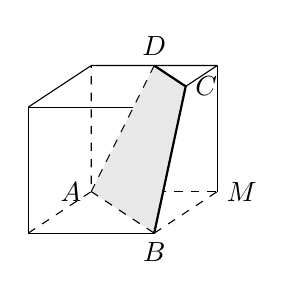
\begin{tikzpicture}[>=stealth, scale=1.6, line join=round]
  % 投影：x 向右、y 向右上（景深）、z 向上
  \def\px#1#2#3{#1+0.5*#2}
  \def\py#1#2#3{#3+0.33*#2}
  % 立方体八个顶点
  \coordinate (FBL) at (0,0);
  \coordinate (BBL) at (0.5,0.33);   % A
  \coordinate (FBR) at (1,0);        % B
  \coordinate (BBR) at (1.5,0.33);   % M
  \coordinate (FTL) at (0,1);
  \coordinate (BTL) at (0.5,1.33);
  \coordinate (FTR) at (1,1);
  \coordinate (BTR) at (1.5,1.33);
  % 可见棱（实线）
  \draw (FBL)--(FBR)--(FTR)--(FTL)--cycle;
  \draw (FTL)--(BTL)--(BTR)--(FTR);
  \draw (BTR)--(BBR);
  % 不可见棱（虚线）
  \draw[dashed] (FBL)--(BBL)--(BTL);
  \draw[dashed] (BBL)--(BBR);
  \draw[dashed] (FBR)--(BBR);
  % 截面：C、D 为两条棱中点，A、B、M 为顶点
  \coordinate (C) at (1.25,1.165);
  \coordinate (D) at (1.0,1.33);
  \fill[gray!18] (0.5,0.33)--(1,0)--(1.25,1.165)--(1.0,1.33)--cycle;
  \draw[dashed] (0.5,0.33)--(1,0);
  \draw[dashed] (0.5,0.33)--(1.0,1.33);
  \draw[thick] (1,0)--(1.25,1.165)--(1.0,1.33);
  % 标注
  \node[left] at (0.5,0.33) {$A$};
  \node[below] at (1,0) {$B$};
  \node[right] at (1.5,0.33) {$M$};
  \node[right] at (1.25,1.165) {$C$};
  \node[above] at (1.0,1.33) {$D$};
\end{tikzpicture}
\end{center}
\nopagebreak[4]
\end{question}
\begin{question}
\gkti{15}用 $1$、$2$、$3$、$4$、$5$、$6$、$7$、$8$ 组成没有重复数字的八位数，要求 $1$ 和 $2$ 相邻，$3$ 与 $4$ 相邻，$5$ 与 $6$ 相邻，而 $7$ 与 $8$ 不相邻，这样的八位数共有 $\underline{\hspace{2cm}}$ 个．（用数字作答）

\end{question}
\begin{question}
\gkti{16}$\omega$ 是正实数，设 $S_\omega = \{\theta \mid f(x) = \cos[\omega(x+\theta)] \text{ \text{是奇函数}}\}$，若对每个实数 $a$，$S_\omega \cap (a, a+1)$ 的元素不超过 $2$ 个，且有 $a$ 使 $S_\omega \cap (a, a+1)$ 含 $2$ 个元素，则 $\omega$ 的取值范围是 $\underline{\hspace{2cm}}$．

\end{question}
\gkpart{三、解答题（本大题共 6 小题，共 74 分．解答应写出文字说明、证明过程或演算步骤）}

\Needspace{0.4\textheight}
\begin{question}
\gkti{17}（本小题满分 12 分）已知三棱锥 $P-ABC$ 中，$E$、$F$ 分别是 $AC$、$AB$ 的中点，$\triangle ABC$、$\triangle PEF$ 都是正三角形，$PF \perp AB$．
\nopagebreak[4]
\begin{center}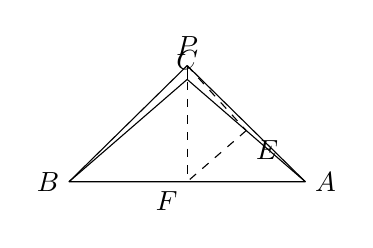
\begin{tikzpicture}[>=stealth, scale=1.5, line join=round]
  % 投影：x 向右，y 向屏幕内（0.5 压缩），z 向上（0.85 压缩）
  \coordinate (A) at (1,0);
  \coordinate (B) at (-1,0);
  \coordinate (C) at (0,0.866);
  \coordinate (F) at (0,0);
  \coordinate (E) at (0.5,0.433);
  \coordinate (P) at (0,0.983);
  % 棱
  \draw (A)--(B)--(C)--cycle;
  \draw (P)--(A);
  \draw (P)--(B);
  \draw (P)--(C);
  % 辅助线（中位线与等边三角形 PEF）
  \draw[dashed] (E)--(F);
  \draw[dashed] (P)--(F);
  \draw[dashed] (P)--(E);
  % 标注
  \node[right] at (A) {$A$};
  \node[left] at (B) {$B$};
  \node[above] at (C) {$C$};
  \node[above] at (P) {$P$};
  \node[below left] at (F) {$F$};
  \node[below right] at (E) {$E$};
\end{tikzpicture}
\end{center}
\nopagebreak[4]
(1) 证明：$PC \perp \text{\text{平面} } PAB$；
(2) 求二面角 $P-AB-C$ 的平面角的余弦值；
(3) 若点 $P$、$A$、$B$、$C$ 在一个表面积为 $12\pi$ 的球面上，求 $\triangle ABC$ 的边长．

\Needspace{0.4\textheight}
\end{question}
\begin{question}
\gkti{18}（本小题满分 12 分）如图，在直径为 $1$ 的圆 $O$ 中，作一关于圆心对称、邻边互相垂直的十字形，其中 $y > x > 0$．
\nopagebreak[4]
\begin{center}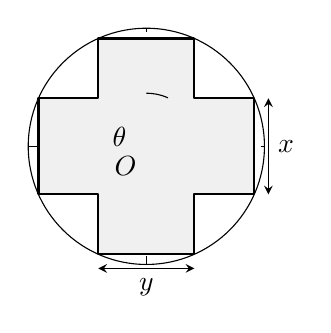
\begin{tikzpicture}[>=stealth, scale=1.5, line join=round]
  \def\th{24}
  \pgfmathsetmacro{\xh}{sin(\th)}
  \pgfmathsetmacro{\yh}{cos(\th)}
  % 圆（直径 1，图中按比例放大）
  \draw (0,0) circle (1);
  \draw[dashed] (-1,0) -- (1,0);
  \draw[dashed] (0,-1) -- (0,1);
  % 十字形
  \draw[thick, fill=gray!12]
    (\yh,\xh) -- (\xh,\xh) -- (\xh,\yh) -- (-\xh,\yh) -- (-\xh,\xh) -- (-\yh,\xh)
    -- (-\yh,-\xh) -- (-\xh,-\xh) -- (-\xh,-\yh) -- (\xh,-\yh) -- (\xh,-\xh) -- (\yh,-\xh) -- cycle;
  % 角 theta
  \draw (0,0.45) arc (90:90-\th:0.45);
  \node at ({0.40*cos(90-\th/2+90)},{0.40*sin(90-\th/2+90)}) [right=1pt] {$\theta$};
  % 尺寸标注
  \draw[<->] (\yh+0.12,-\xh) -- (\yh+0.12,\xh) node[midway,right] {$x$};
  \draw[<->] (-\xh,-\yh-0.12) -- (\xh,-\yh-0.12) node[midway,below] {$y$};
  \node[below left] at (0,0) {$O$};
\end{tikzpicture}
\end{center}
\nopagebreak[4]
(1) 将十字形的面积表示为 $\theta$ 的函数；
(2) $\theta$ 为何值时，十字形的面积最大？最大面积是多少？

\end{question}
\begin{question}
\gkti{19}（本小题满分 12 分）已知函数 $f(x) = \dfrac{x+3}{x+1}$（$x \neq -1$）．设数列 $\{a_n\}$ 满足 $a_1 = 1$，$a_{n+1} = f(a_n)$，数列 $\{b_n\}$ 满足 $b_n = |a_n - \sqrt{3}|$，$S_n = b_1 + b_2 + \cdots + b_n$（$n \in \mathbf{N}^*$）．

(1) 用数学归纳法证明：$b_n \leqslant \dfrac{(\sqrt{3}-1)^n}{2^{n-1}}$；
(2) 证明：$S_n < \dfrac{2\sqrt{3}}{3}$．

\end{question}
\begin{question}
\gkti{20}（本小题满分 12 分）某工厂生产甲、乙两种产品，每种产品都是经过第一和第二工序加工而成，两道工序的加工结果相互独立，每道工序的加工结果均有 A、B 两个等级．对每种产品，两道工序的加工结果都为 A 级时，产品为一等品，其余均为二等品．

(1) 已知甲、乙两种产品每一道工序的加工结果为 A 级的概率如表一所示，分别求生产出的甲、乙产品为一等品的概率 $P_\text{\text{甲}}$、$P_\text{\text{乙}}$；

表一

\begin{center}
\begin{tabular}{lcc}
\toprule
概率 \ 工序 & 第一工序 & 第二工序 \\
\midrule
甲 & 0.8 & 0.85 \\
乙 & 0.75 & 0.8 \\
\bottomrule
\end{tabular}
\end{center}

(2) 已知一件产品的利润如表二所示，用 $\xi$、$\eta$ 分别表示一件甲、乙产品的利润，在 (1) 的条件下，求 $\xi$、$\eta$ 的分布列及 $E\xi$、$E\eta$；

表二

\begin{center}
\begin{tabular}{lcc}
\toprule
利润 \ 等级 & 一等 & 二等 \\
\midrule
甲 & 5（万元） & 2.5（万元） \\
乙 & 2.5（万元） & 1.5（万元） \\
\bottomrule
\end{tabular}
\end{center}

(3) 已知生产一件产品需用的工人数和资金额如表三所示．该工厂有工人 40 名，可用资金 60 万元．设 $x$、$y$ 分别表示生产甲、乙产品的数量，在 (2) 的条件下，$x$、$y$ 为何值时，$z = xE\xi + yE\eta$ 最大？最大值是多少？

表三

\begin{center}
\begin{tabular}{lcc}
\toprule
用量 \ 项目 & 工人（名） & 资金（万元） \\
\midrule
甲 & 8 & 8 \\
乙 & 2 & 10 \\
\bottomrule
\end{tabular}
\end{center}

\Needspace{0.4\textheight}
\end{question}
\begin{question}
\gkti{21}（本小题满分 14 分）已知椭圆 $\dfrac{x^2}{a^2} + \dfrac{y^2}{b^2} = 1$（$a > b > 0$）的左、右焦点分别是 $F_1(-c, 0)$、$F_2(c, 0)$，$Q$ 是椭圆外的动点，满足 $\overrightarrow{F_1Q} = 2a$．点 $P$ 是线段 $F_1Q$ 与该椭圆的交点，点 $T$ 在线段 $F_2Q$ 上，并且满足 $\overrightarrow{PT} \cdot \overrightarrow{TF_2} = 0$，$\overrightarrow{TF_2} \neq 0$．
\nopagebreak[4]
\begin{center}\begin{tikzpicture}[>=stealth, scale=1.3, line join=round]
  % 椭圆
  \draw[thick] (0,0) ellipse (2.2 and 1.35);
  \coordinate (F1) at (-1.6,0);
  \coordinate (F2) at (1.6,0);
  \fill (F1) circle (1.2pt) node[below] {$F_1$};
  \fill (F2) circle (1.2pt) node[below] {$F_2$};
  % 外部点 Q 与线段 F1Q、F2Q
  \coordinate (Q) at (3.1,2.1);
  \fill (Q) circle (1.2pt) node[above right] {$Q$};
  \draw (F1)--(Q);
  \draw (F2)--(Q);
  % 交点 P（在椭圆上、线段 F1Q 上）
  \coordinate (P) at (0.62,1.25);
  \fill (P) circle (1.2pt) node[above left] {$P$};
  % T 为 F2Q 中点，PT 垂直于 F2Q
  \coordinate (T) at ({0.5*(1.6+3.1)},{0.5*2.1});
  \fill (T) circle (1.2pt) node[right] {$T$};
  \draw (P)--(T);
  % 直角标记
  \draw[thick] ($(T)!0.09!(P)$) -- ($(T)!0.09!(Q)$) -- ($(T)!0.09!(Q)+(T)!0.09!(P)-(T)$);
\end{tikzpicture}
\end{center}
\nopagebreak[4]
(1) 设 $x$ 为点 $P$ 的横坐标，证明：$\overrightarrow{F_1P} = a + \dfrac{c}{a}x$；
(2) 求点 $T$ 的轨迹 $C$ 的方程；
(3) 试问：在点 $T$ 的轨迹 $C$ 上，是否存在点 $M$，使 $\triangle F_1MF_2$ 的面积 $S = b^2$．若存在，求 $\angle F_1MF_2$ 的正切值；若不存在，请说明理由．

\end{question}
\begin{question}
\gkti{22}（本小题满分 12 分）函数 $y = f(x)$ 在区间 $(0, +\infty)$ 内可导，导函数 $f'(x)$ 是减函数，且 $f'(x) > 0$．设 $x_0 \in (0, +\infty)$，$y = kx + m$ 是曲线 $y = f(x)$ 在点 $(x_0, f(x_0))$ 处的切线方程，并设函数 $g(x) = kx + m$．

(1) 用 $x_0$、$f(x_0)$、$f'(x_0)$ 表示 $m$；
(2) 证明：当 $x_0 \in (0, +\infty)$，$g(x) \geqslant f(x)$；
(3) 若关于 $x$ 的不等式 $x^2 + 1 \geqslant ax + b \geqslant \dfrac{3}{2}x^{\frac{2}{3}}$ 在 $[0, +\infty)$ 上恒成立，其中 $a$、$b$ 为实数，求 $b$ 的取值范围及 $a$ 与 $b$ 所满足的关系．

\end{question}